\documentclass[12pt,a4paper]{book}

\usepackage{geometry}
\usepackage{amsmath,amssymb}

\usepackage{xcolor}

\usepackage{tikz,pgfplots}
\pgfplotsset{compat=1.12}
\usepgfplotslibrary{fillbetween}
\usetikzlibrary{patterns}
\usetikzlibrary{positioning}
\usetikzlibrary{arrows,automata,shapes}
\usepackage[skip=2pt]{caption}
\newcommand\encircle[1]{%
  \tikz[baseline=(X.base)] 
    \node (X) [draw, shape=circle, inner sep=0] {\strut #1};}

\begin{document}
page $109$\\\\
\begin{center}
\begin{tikzpicture}[shorten >=1pt,node distance=5cm,on grid,auto]
  \node[state] (b1)  [align=center] {$B_1$ \\ $1$ };
  \node[state](b0) [below of=b1,align=center] {$B_0$ \\ $0$};
   \node[initial,state,initial text=] (a) [left=of b0,align=center] {$A$ \\ $0$}; 
   \node[state] (c) [ right=of b0] {$C$}; 
    \node[state](d) [below=of b0] {$D$};
   \draw[->] (a) edge node {a} (b0);
   \draw[->] (a) edge [bend left=10] node[above] {b/0} (d);
   \draw[->] (d) edge [bend left=10] node [below] {a} (a);
   \draw[->] (c) edge node {a/0} (d);
   \draw[->] (b0) edge node [below] {b/0} (c);
   \draw[->] (c) edge node [below] {b} (b1);
   \draw[->] (b0) edge  node {a} (b1);
   \draw[->] (d) edge [loop below ] node {b/1} (d);
   \draw [->] (b1) -|  node[above left]{b/0}  (c);
   \draw[->] (b1) edge [loop above] node  {a} (b1);
 \end{tikzpicture}
 \end{center}
For the state A, the incoming edges to this state are from $B_0$ to C with label $b/0$ and$ B_1$ to C with
label $b/0$. There is no difference in the outputs of the incoming edges to this state, and so in the
constructing Moore machine the output for this state will be $0$. \newpage
\begin{center}
\begin{tikzpicture}[shorten >=1pt,node distance=5cm,on grid,auto]
  \node[state] (b1)  [align=center] {$B_1$ \\ $1$ };
  \node[state](b0) [below of=b1,align=center] {$B_0$ \\ $0$};
   \node[initial,state,initial text=] (a) [left=of b0,align=center] {$A$ \\ $0$}; 
   \node[state] (c) [ right=of b0,align=center] {$C$\\$0$}; 
    \node[state](d) [below=of b0] {$D$};
   \draw[->] (a) edge node {a} (b0);
   \draw[->] (a) edge [bend left=10] node[above] {b/0} (d);
   \draw[->] (d) edge [bend left=10] node [below] {a} (a);
   \draw[->] (c) edge node {a/0} (d);
   \draw[->] (b0) edge node [below] {b} (c);
   \draw[->] (c) edge node [below] {b} (b1);
   \draw[->] (b0) edge  node {a} (b1);
   \draw[->] (d) edge [loop below ] node {b/1} (d);
   \draw [->] (b1) -|  node[above left]{b}  (c);
   \draw[->] (b1) edge [loop above] node  {a} (b1);
 \end{tikzpicture}
 \end{center}
For the state D, the incoming edges are A to D with label $b/0$, from C to D with label $a/0$, and
from D to D with label $b/1$.\\
We get two different outputs for two incoming edges $($D to D output $1$, C to D output $0)$.\\
So, the state D will be divided into two, namely, $D_0$ and $D_1$. The outgoing edges are duplicated
for both the states generated from D. The modifi ed machine is 
\begin{center}
\begin{tikzpicture}[shorten >=1pt,node distance=5cm,on grid,auto]
  \node[state] (b1)  [align=center] {$B_1$ \\ $1$ };
  \node[state](b0) [below of=b1,align=center] {$B_0$ \\ $0$};
   \node[initial,state,initial text=] (a) [left=of b0,align=center] {$A$ \\ $0$}; 
   \node[state] (c) [ right=of b0,align=center] {$C$\\$0$}; 
    \node[state](d) [below=of b0,align=center] {$D_0$ \\ $0$};
    \node[state](d1) [below left=of d,align=center] {$D_1$ \\ $1$};
   \draw[->] (a) edge node {a} (b0);
   \draw[->] (a) edge [bend left=10] node[above] {b} (d);
   \draw[->] (d) edge [bend left=10] node [below] {a} (a);
   \draw[->] (c) edge node {a} (d);
   \draw[->] (b0) edge node [below] {b} (c);
   \draw[->] (c) edge node [below] {b} (b1);
   \draw[->] (b0) edge  node {a} (b1);
   \draw[->] (d1) edge [loop below ] node {b} (d1);
   \draw [->] (b1) -|  node[above left]{b}  (c);
   \draw[->] (b1) edge [loop above] node  {a} (b1);
   \draw [->] (d1) -|  node[left]{a}  (a);
   \draw[->] (d) edge  node {b} (d1);
 \end{tikzpicture}
 \end{center} \newpage
 page $110$\\\\
 $21.$ Convert the following Mealy machine into an equivalent Moore machine. $\left[UPTU 2004\right]$.\\
Solution: The state $q_0$ has two incoming edges: from $q_1$ with label $a/0$ and from $q_3$ with label $b/1$. As there is a difference in output, the state $q_0$ is divided into $q_{00}$ and $q_{01}$ with outputs $0$ and $1$, respectively.\\
The states $q_1$ and $q_3$ have only one incoming edge each, and so there is no need of division.\\
The state $q_2$ has three incoming edges; among those, two are of output $'0'$ and another is of output $'1'$.\\
Thus, it is divided into $q_{20}$ and $q_{21}$ with outputs $0$ and $1$,respectively.\vspace*{-3mm}.
\begin{center}
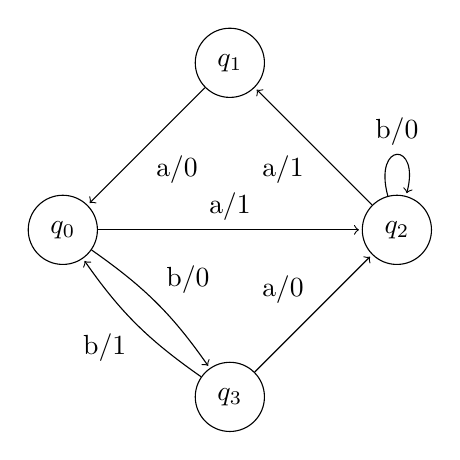
\begin{tikzpicture}[shorten >=1pt,node distance=3cm,on grid,auto]
  \node[state] (q0)   {$q_0$}; 
   \node[state] (q1) [above right=of q0] {$q_1$}; 
   \node[state] (q2) [below right=of q1] {$q_2$}; 
   \node[state](q3) [below right=of q0] {$q_3$};
   \path[->] (q0) edge node {a/1} (q2);
   \path[->] (q1) edge node {a/0} (q0);
   \path[->] (q2) edge node {a/1} (q1);
   \path[->] (q3) edge node {a/0} (q2);
   \path[->] (q3) edge [bend left=10] node [below left] {b/1} (q0);
   \path[->] (q0) edge [bend left=10] node {b/0} (q3);
   \path[->] (q2) edge [loop above] node {b/0} (q2);
 \end{tikzpicture}
 \end{center}\vspace*{-3mm}.
From $q_1$ input with label ‘a’ ends on $q_0$0, and from $q_3$ input with label ‘b’ ends on $q_0$1. The outputs from old $q_1$ state are duplicated from $q_0$0 and $q_0$1. The state $q_1$ and $q_3$ are not divided.\\
$q_1$ gets output $'1'$ and $q_3$ gets output $'0'$. Dividing the state $q_0$ and placing $q_1$ and $q_3$, the intermediate machine becomes as follows.\vspace*{-2mm}.
\begin{center}
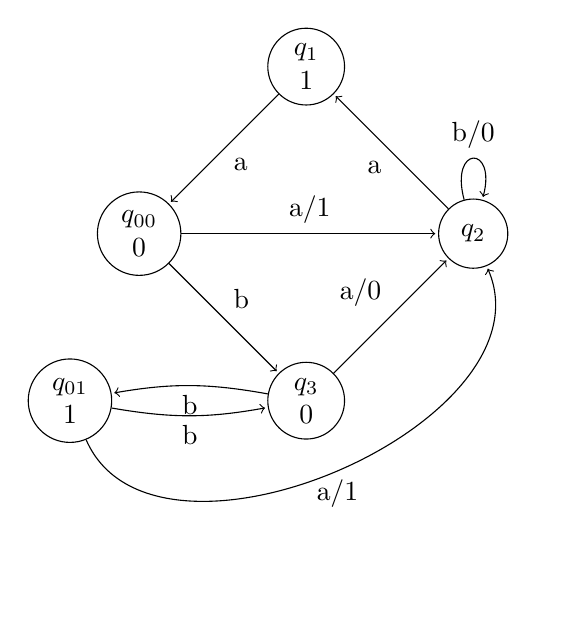
\begin{tikzpicture}[shorten >=1pt,node distance=3cm,on grid,auto]
  \node[state] (q0)  [align=center] {$q_{00}$ \\ $0$}; 
   \node[state] (q1) [above right=of q0,align=center] {$q_1$ \\ $1$}; 
   \node[state] (q2) [below right=of q1] {$q_2$}; 
   \node[state](q3) [below left=of q2,align=center] {$q_3$ \\ 0};
   \node[state](q4) [left of=q3,align=center] {$q_{01}$ \\ $1$};
   \draw[->] (q0) edge node {a/1} (q2);
   \draw[->] (q1) edge node {a} (q0);
   \draw[->] (q2) edge node {a} (q1);
   \draw[->] (q3) edge node {a/0} (q2);
   \draw[->] (q3) edge [bend right=10] node [below] {b} (q4);
   \draw[->] (q4) edge [bend right=10] node [below] {b} (q3);
   \draw[->] (q0) edge  node [above right] {b} (q3);
   \draw[->] (q2) edge [loop above] node {b/0} (q2);
   \draw[->] (q4) edge [bend right=90] node [below] {a/1} (q2);
 \end{tikzpicture}
 \end{center}\vspace*{-2mm}.
The state $q_2$ is divided into $q_{20}$ and $q_{21}$. From $q_{00}$ and $q_{01}$ input with label $'a'$ ends on $q_{21}$. From $q_3$ input with label $'a'$ ends on $q_{20}$. There is a loop on $q_2$. That loop will be on $q_{20}$ with label $'b'$. Another transition with label $'b'$ is drawn from $q_{21}$ to $q_{20}$. The fi nal Moore machine is as follows.\vspace*{-3mm}.
\begin{center}
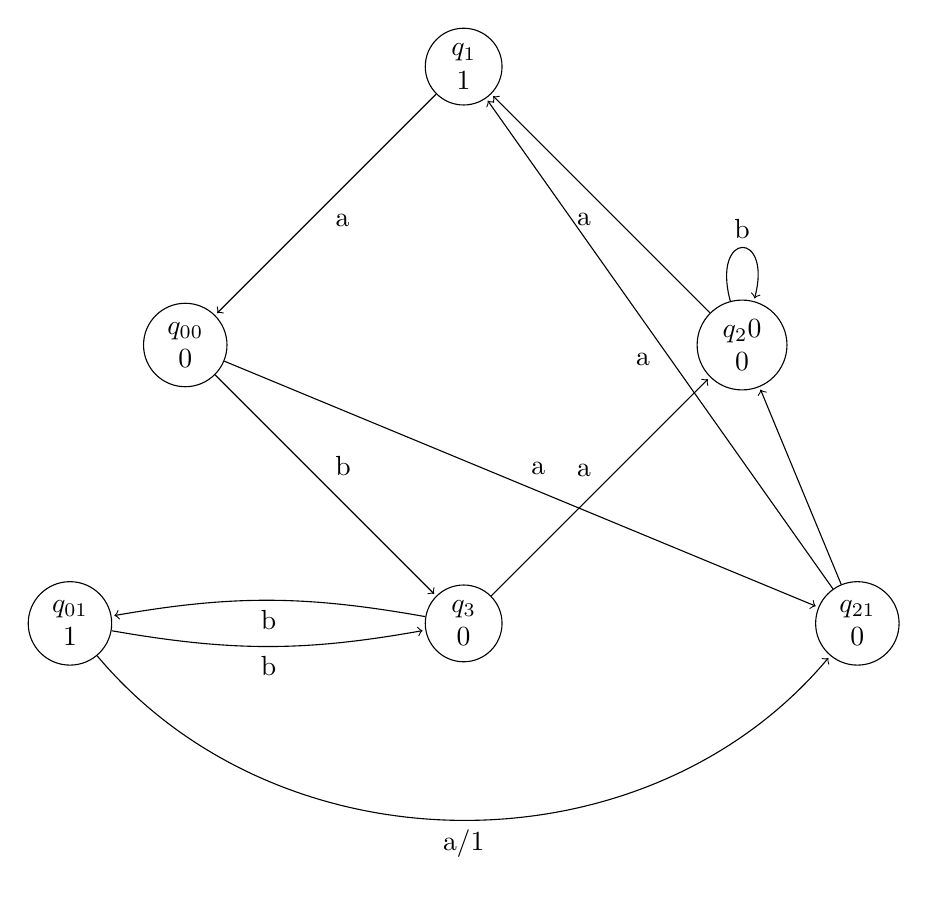
\begin{tikzpicture}[shorten >=1pt,node distance=5cm,on grid,auto]
  \node[state] (q0)  [align=center] {$q_{00}$ \\ $0$}; 
   \node[state] (q1) [above right=of q0,align=center] {$q_1$ \\ $1$}; 
   \node[state] (q2) [below right=of q1,align=center] {$q_20$\\$0$}; 
   \node[state](q3) [below left=of q2,align=center] {$q_3$ \\ 0};
   \node[state](q4) [left of=q3,align=center] {$q_{01}$ \\ $1$};
   \node[state](q5) [right of=q3,align=center] {$q_{21}$ \\ $0$};
   \draw[->] (q0) edge node {a} (q5);
   \draw[->] (q1) edge node {a} (q0);
   \draw[->] (q2) edge node {a} (q1);
   \draw[->] (q3) edge node {a} (q2);
   \draw[->] (q3) edge [bend right=10] node [below] {b} (q4);
   \draw[->] (q4) edge [bend right=10] node [below] {b} (q3);
   \draw[->] (q0) edge  node [above right] {b} (q3);
   \draw[->] (q2) edge [loop above] node {b} (q2);
   \draw[->] (q4) edge [bend right=50] node [below] {a/1} (q5);
   \draw[->] (q5) edge node {} (q2);
   \draw[->] (q5) edge node {a} (q1);
\end{tikzpicture}
\end{center}\newpage
page $111$\\\\
$22.$ Minimize the following fi nite automata.\\
\begin{center}
\begin{table}[h]
\centering
\scalebox{2}{
\begin{tabular}{llr}
\hline
&\multicolumn{2}{c}{Next State} \\
\cline{2-3}
\centering
Present State   &I/P = a & I/P = b \\
\hline
$\rightarrow$A      &B    &F      \\
B &A &F \\
C &G &A \\
D &H &B\\
E &A &G\\
F &H &C\\
G &A &D\\
H &A &C\\
\hline
\end{tabular}
}
\end{table}
\end{center}
Here F, G, and H are the fi nal states.\\
Solution: In the fi nite automata, the states are $\{A, B, C, D, E, F, G, H\}$. Name this set as $S_0$.\\
$S_0: \{A, B, C, D, E, F, G, H\}$\\
All of the states are 0 equivalents.\\
In the fi nite automata, there are two types of states: fi nal state and non-fi nal states. So, divide
the set of states into two parts, $Q_1$ and $Q_1$.\\
$Q_1 = \{F, G, H\} \quad \quad Q_2 = \{A, B, C, D, E\}$\\
$S_1: \{\{F, G, H\} \{A, B, C, D, E\}\}$\\
The states belonging to same subset are 1-equivalent because they are in the same set for string
length 1. The states belonging to different subsets are 1-distinguishable.\\
The next states of F are H and C. The next states of G and H are A, D and A, C, respectively.\\
A, D and A, C belong to the same subset but H and C belong to a different subset. So, F, G, and
H are divided into $\{F\}, \{G, H\}$.\\
For input 0, the next states of A, B, C, D, and E are B, A, G, H, and A, respectively. For input 1,
the next states of A, B, C, D, and E are F, F, A, B, and G, respectively. So, the set ${A, B, C, D, E}$
is divided into $\{A, B, E\}$ and $\{C, D\}$.\\
$S_2: \{\{F\} \{G, H\} \{A, B, E\} \{C, D\}\}$\\
By the same process, $\{A, B, E\}$ is divided into $\{A, B\}, \{E\}$.\\
$S_3: \{\{F\} \{G, H\} \{A, B\} \{E\} \{C, D\}\} = \{\{A, B\}, \{C, D\},\{E\}, \{F\}, \{G, H\}\}$\\
The set is not dividable further. So, these are the states of minimized DFA. Let us rename the
subsets as $q_0$, $q_1$, $q_2$, $q_3$, and $q_4$. The initial state was A, and so here the initial state is {A, B}, i.e., $q_0$.\\
The fi nal state was F, G, and H, and so here the fi nal states are $\{F\}$, i.e., $q_3$ and $\{G, H\}$, i.e., $q_4$.
The tabular representation of minimized DFA is \newpage
page $112$\\\\
\begin{center}
\begin{table}[h]
\centering
\scalebox{2}{
\begin{tabular}{llr}
\hline
&\multicolumn{2}{c}{Next State} \\
\cline{2-3}
\centering
Present State   &I/P = 0 & I/P = 1 \\
\hline
$\rightarrow q_0$      &$q_0$    &$q_3$      \\
$q_1$ &$q_4$ &$q_0$ \\
$q_2$ &$q_0$ &$q_4$ \\
\encircle{$q_3$} &$q_4$ &$q_1$\\
\encircle{$q_4$} &$q_0$ &$q_1$\\
\hline
\end{tabular}
}
\end{table}
\end{center}
$23.$ Design a Mealy and Moore machine for detecting a sequence 1010 where overlapping sequences
are also accepted. Convert the Moore machine that you have got into a Mealy machine. Are there
any differences? How will you prove that the two Mealy machines are equivalent?\\
\textbf{Solution:} The Mealy machine is
\begin{center}
\begin{tikzpicture}[shorten >=1pt,node distance=5cm,on grid,auto]
   \node[state] (a)  {$A$}; 
   \node[state] (b) [ right=of a] {$B$}; 
   \node[state] (c) [ right=of b] {$C$}; 
   \node[state] (d) [ right=of c] {$D$}; 
   \draw[->] (a) edge node {1/0} (b);
   \draw[->] (d) edge [bend right=40] node[above] {1/0} (b);
   \draw[->] (c) edge [bend left=60] node [below] {0/0} (a);
   \draw[->] (b) edge node {0/0} (c);
   \draw[->] (c) edge node {1/0} (d);
   \draw[->] (d) edge [bend left=30] node [below] {0/1} (c);
   \draw[->] (a) edge [loop above] node {0/0} (a); 
   \draw[->] (b) edge [loop above] node  {1/0} (b);
 \end{tikzpicture}
 \end{center}
 The Moore machine is\\
\begin{center}
\begin{tikzpicture}[shorten >=1pt,node distance=3.6cm,on grid,auto]
   \node[state] (a)  {$A/0$}; 
   \node[state] (b) [ right=of a] {$B/0$}; 
   \node[state] (c) [ right=of b] {$C/0$}; 
   \node[state] (d) [ right=of c] {$D/0$}; 
   \node[state] (e) [ right=of d] {$E/1$}; 
   \draw[->] (a) edge node {1} (b);
   \draw[->] (d) edge [bend right=40] node[above] {1} (b);
   \draw[->] (e) edge [bend right=50] node[above] {0} (a);
   \draw[->] (c) edge [bend left=50] node [below] {0} (a);
   \draw[->] (b) edge node {0} (c);
   \draw[->] (c) edge node {1} (d);
   \draw[->] (d) edge node {0} (e);
   \draw[->] (d) edge [bend left=30] node [below] {0/1} (c);
   \draw[->] (e) edge [bend left=30] node [below] {1} (d);
   \draw[->] (a) edge [loop above] node {0} (a); 
   \draw[->] (b) edge [loop above] node  {1} (b);
 \end{tikzpicture}
 \end{center} 
The converted Mealy machine from the given Moore machine is (by using the transactional
format)
\begin{center}
\begin{tikzpicture}[shorten >=1pt,node distance=3.6cm,on grid,auto]
   \node[state] (a)  {$A$}; 
   \node[state] (b) [ right=of a] {$B$}; 
   \node[state] (c) [ right=of b] {$C$}; 
   \node[state] (d) [ right=of c] {$D$}; 
   \node[state] (e) [ right=of d] {$E$}; 
   \draw[->] (a) edge node {1/0} (b);
   \draw[->] (d) edge [bend right=40] node[above] {1/0} (b);
   \draw[->] (e) edge [bend right=50] node[above] {0/0} (a);
   \draw[->] (c) edge [bend left=50] node [below] {0/0} (a);
   \draw[->] (b) edge node {0/0} (c);
   \draw[->] (c) edge node {1/0} (d);
   \draw[->] (d) edge node {0/1} (e);
   \draw[->] (d) edge [bend left=30] node [below] {0/1} (c);
   \draw[->] (e) edge [bend left=30] node [below] {1/0} (d);
   \draw[->] (a) edge [loop above] node {0/0} (a); 
   \draw[->] (b) edge [loop above] node  {1/0} (b);
 \end{tikzpicture}
 \end{center} 
\end{document}